\section*{\textkhmer{មេរៀនទី ១: ចំនួនគត់ធម្មជាតិ}}\label{sec:textkhmer{--------}}

\subsection*{វត្ថុបំណងនៃការសិក្សា}
    នៅចុងបញ្ចប់នៃមេរៀននេះ សិស្សនឹងអាច៖
    \begin{itemize}[label=-]
        \item កំណត់និយមន័យចំនួនគត់ធម្មជាតិ និងតាងវានៅលើបន្ទាត់ចំនួន។
        \item ប្រើតម្លៃខ្ទង់ដើម្បីអាន សរសេរ និងពន្លាតចំនួនគត់ធម្មជាតិ។
        \item ប្រៀបធៀប និងរៀបលំដាប់ចំនួនគត់ធម្មជាតិដោយប្រើ $<, >,$ និង $=$.
        \item អនុវត្តប្រមាណវិធីទាំងបួន (បូក ដក គុណ ចែក) ជាមួយចំនួនគត់ធម្មជាតិ។
        \item ប្រើលក្ខណៈនៃប្រមាណវិធី (លក្ខណៈត្រឡប់, លក្ខណៈផ្ដុំ, លក្ខណៈបំបែក)។
        \item កំណត់កត្តា និងពហុគុណ; ចំណាត់ថ្នាក់ចំនួនជាចំនួនបឋម ឬចំនួនមិនបឋម។
        \item អនុវត្តវិធានចែកដាច់ជាមូលដ្ឋាន ($2, 3, 5, 9, 10$)។
    \end{itemize}

\section{គោលគំនិតសំខាន់ៗ}
\subsection{តើអ្វីជាចំនួនគត់ធម្មជាតិ?}
ចំនួនគត់ធម្មជាតិគឺជាចំនួនរាប់៖ $\{1,2,3,4,\dots\}$ ។ ក្នុងបរិបទខ្លះ លេខ $0$ ក៏ត្រូវបានរួមបញ្ចូលដែរ ដែលតាងដោយ $\mathbb{N}_0 = \{0, 1, 2, 3, \dots\}$។ នៅក្នុងមេរៀននេះ យើងប្រើ $\mathbb{N}=\{1,2,3,\dots\}$ លុះត្រាតែបានបញ្ជាក់ផ្សេងពីនេះ។

\subsection{បន្ទាត់ចំនួន}
ចំនួនគត់ធម្មជាតិមានគម្លាតស្មើៗគ្នានៅលើបន្ទាត់ចំនួននៅខាងស្ដាំនៃលេខ $0$។
\begin{figure}[h!]
    \centering
    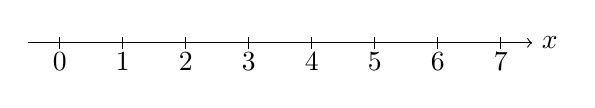
\begin{tikzpicture}[scale=0.8]
        \draw[->] (-0.5,0) -- (7.5,0) node[right] {$x$};
        \foreach \x in {0,1,2,3,4,5,6,7} {
            \draw (\x, -0.1) -- (\x, 0.1);
            \node at (\x, -0.3) {\x};
        }
    \end{tikzpicture}
    \caption{បន្ទាត់ចំនួនបង្ហាញពីទីតាំងនៃចំនួនគត់ធម្មជាតិ។}
    \label{fig:number-line}
\end{figure}

\subsection{តម្លៃខ្ទង់ និងទម្រង់ពន្លាត}
គ្រប់ខ្ទង់ទាំងអស់មានតម្លៃតាមខ្ទង់របស់វា។ ឧទាហរណ៍ $53\,407$:
    \[
        53\,407 = 5\times10^4 + 3\times10^3 + 4\times10^2 + 0\times10^1 + 7\times10^0.
    \]

\subsection{ការប្រៀបធៀប និងការរៀបលំដាប់}
ដើម្បីប្រៀបធៀបចំនួន ត្រូវប្រៀបធៀបខ្ទង់ពីឆ្វេងទៅស្តាំ (តម្លៃខ្ទង់ខ្ពស់បំផុតមុនគេ)។ ប្រើសញ្ញា $>$ (ធំជាង), $<$ (តូចជាង), និង $=$ (ស្មើ)។

\subsection{ប្រមាណវិធី និងលក្ខណៈ}
    \begin{itemize}[label=---,nosep]
        \item លក្ខណៈត្រឡប់៖ $a+b=b+a$, $ab=ba$។
        \item លក្ខណៈផ្ដុំ៖ $(a+b)+c=a+(b+c)$, $(ab)c=a(bc)$។
        \item លក្ខណៈបំបែក៖ $a(b+c)=ab+ac$។
    \end{itemize}

\subsection{កត្តា, ពហុគុណ, ចំនួនបឋម និងចំនួនមិនបឋម}
    \begin{itemize}[label=---,nosep]
        \item កត្តានៃ $n$ គឺជាចំនួនដែលចែក $n$ ដាច់។
        \item ពហុគុណនៃ $n$ គឺ $n\times k$ ដែល $k$ ជាចំនួនគត់ធម្មជាតិណាមួយ។
        \item ចំនួនបឋមមានកត្តាពីរគត់គឺ 1 និងខ្លួនវា (ឧ., 2, 3, 5, 7, 11)។
        \item ចំនួនមិនបឋមមានកត្តាច្រើនជាងពីរ (ឧ., 4, 6, 8, 9, 10)។
    \end{itemize}

\subsection{វិធាននៃការចែកដាច់}
    \begin{itemize}[label=-]
        \item 2: ខ្ទង់ចុងក្រោយជាចំនួនគូ។
        \item 3: សរុបផលបូកនៃខ្ទង់ទាំងអស់ចែកដាច់នឹង 3។
        \item 5: ខ្ទង់ចុងក្រោយគឺ 0 ឬ 5។
        \item 9: សរុបផលបូកនៃខ្ទង់ទាំងអស់ចែកដាច់នឹង 9។
        \item 10: ខ្ទង់ចុងក្រោយគឺ 0។
    \end{itemize}

\section{ឧទាហរណ៍អនុវត្ត}

\begin{example}{តម្លៃខ្ទង់}
សរសេរ $608\,305$ ក្នុងទម្រង់ពន្លាត។
\begin{solution}
$608\,305 = 6\times10^5 + 0\times10^4 + 8\times10^3 + 3\times10^2 + 0\times10^1 + 5\times10^0$។
\end{solution}
\end{example}

\begin{example}{ការប្រៀបធៀប}
តើមួយណាធំជាង, $79\,042$ ឬ $78\,904$?
\begin{solution}
ប្រៀបធៀបខ្ទង់ម៉ឺន (ទាំងពីរគឺ 7), ខ្ទង់ពាន់៖ $9>8$, ដូច្នេះ $79\,042>78\,904$។
\end{solution}
\end{example}

\begin{example}{លក្ខណៈ}
គណនាតាមលក្ខណៈបំបែក៖ $27\times 14$។
\begin{solution}
$27\times(10+4)=27\times10+27\times4=270+108=378$។
\end{solution}
\end{example}

\begin{example}{ចំនួនបឋម}
    តើ $91$ ជាចំនួនបឋមឬ?
    \begin{solution}
    ចម្លើយ៖ សាកល្បងជាមួយចំនួនបឋមតូចៗ៖ មិនមែនជាចំនួនគូ, ផលបូកខ្ទង់ $=10$ (មិនចែកដាច់នឹង 3), ខ្ទង់ចុងក្រោយមិនមែន 5 ឬ 0។ សាកល្បង 7: $91\div7=13$។ ដូច្នេះ $91$ ជាចំនួនមិនបឋម៖ $7\times13$។
    \end{solution}
\end{example}

    \section{លំហាត់អនុវត្ត}
    បង្ហាញការគណនារបស់អ្នក។ កន្លែងណាដែលសមរម្យ សូមប្រើតម្លៃខ្ទង់ លក្ខណៈ ឬវិធាននៃការចែកដាច់។

    \subsection*{ក. តម្លៃខ្ទង់ និងទម្រង់ពន្លាត}
    \begin{enumerate}[label=\arabic*.]
        \item សរសេរក្នុងទម្រង់ពន្លាត៖ $40\,706$។
        \item តើខ្ទង់ណានៅក្នុងខ្ទង់ពាន់នៃ $3\,508\,149$?
        \item សរសេរចំនួនដែលមាន 8 នៅខ្ទង់ម៉ឺន, 0 នៅខ្ទង់ពាន់, 6 នៅខ្ទង់រយ, 3 នៅខ្ទង់ដប់, និង 2 នៅខ្ទង់ឯកតា។
    \end{enumerate}

    \subsection*{ខ. ការប្រៀបធៀប និងការរៀបលំដាប់}
    \begin{enumerate}[label=\arabic*.]
        \item ប្រើ $<,>,=$ ដើម្បីប្រៀបធៀប៖ $504\,080\;\_\;503\,890$។
        \item រៀបលំដាប់ពីតូចទៅធំ៖ $9\,805,\;9\,850,\;9\,580$។
        \item តើមួយណាធំជាង៖ $100\,000-1$ ឬ $99\,000+999$?
    \end{enumerate}

    \subsection*{គ. ប្រមាណវិធី}
    \begin{multicols}{2}
        \begin{enumerate}[label=\arabic*.]
            \item $6\,483 + 2\,759$
            \item $12\,000 - 7\,856$
            \item $304\times 25$ (ប្រើលក្ខណៈបំបែក)
            \item $8\,190\div 15$ (បង្ហាញការចែកវែង)
        \end{enumerate}
    \end{multicols}

    \subsection*{ឃ. កត្តា, ពហុគុណ, និងចំនួនបឋម}
    \begin{enumerate}[label=\arabic*.]
        \item រាយកត្តាទាំងអស់នៃ $36$។
        \item តើ $97$ ជាចំនួនបឋម ឬមិនបឋម? ពន្យល់។
        \item រកពហុគុណរួមតូចបំផុត (LCM) នៃ $12$ និង $18$។
        \item រកកត្តារួមធំបំផុត (GCF) នៃ $24$ និង $30$។
    \end{enumerate}

    \subsection*{ង. វិធាននៃការចែកដាច់}
    \begin{enumerate}[label=\arabic*.]
        \item ដោយមិនចាំបាច់ធ្វើការចែក, កំណត់ថាតើ $123\,456$ ចែកដាច់នឹង 3 និង 9 ដែរឬទេ។
        \item តើ $250$ ចែកដាច់នឹងចំនួនណាខ្លះ៖ $2,3,5,6,9,10$? បង្ហាញហេតុផល។
    \end{enumerate}

    \section*{សន្លឹកកិច្ចការបញ្ចប់មេរៀន}
    \begin{enumerate}[label=\arabic*.]
        \item សរសេរ $705\,060$ ជាពាក្យ។
        \item គូសរង្វង់៖ បឋម ឬ មិនបឋម សម្រាប់ $121$។
    \end{enumerate}

\section*{ចម្លើយ (សម្រាប់គ្រូ)}

\begin{multicols}{2}
    \subsection*{ក. តម្លៃខ្ទង់}
    \begin{enumerate}[label=\arabic*.]
        \item $4\times10^4 + 7\times10^2 + 6$
        \item ខ្ទង់ពាន់គឺ 8
        \item $80\,632$
    \end{enumerate}

    \subsection*{ខ. ការប្រៀបធៀប}
    \begin{enumerate}[label=\arabic*.]
        \item $504\,080 > 503\,890$
        \item $9\,580 < 9\,805 < 9\,850$
        \item ស្មើគ្នា ($99\,999$)
    \end{enumerate}

    \subsection*{គ. ប្រមាណវិធី}
    \begin{enumerate}[label=\arabic*.]
        \item $9\,242$
        \item $4\,144$
        \item $7\,600$
        \item $546$
    \end{enumerate}

    \subsection*{ឃ. កត្តា និងចំនួនបឋម}
    \begin{enumerate}[label=\arabic*.]
        \item $1, 2, 3, 4, 6, 9, 12, 18, 36$
        \item បឋម (គ្មានកត្តាចែក)
        \item $\mathrm{LCM}(12,18)=36$
        \item $\mathrm{GCF}(24,30)=6$
    \end{enumerate}

    \subsection*{ង. វិធានចែកដាច់}
    \begin{enumerate}[label=\arabic*.]
        \item ដាច់នឹង 3, មិនដាច់នឹង 9
        \item $2, 5, 10$
    \end{enumerate}

    \subsection*{បញ្ចប់មេរៀន}
    \begin{enumerate}[label=\arabic*.]
        \item ប្រាំពីររយប្រាំពាន់ហុកសិប
        \item មិនបឋម ($11\times11$)
    \end{enumerate}
\end{multicols}
